\begin{figure}[!h]
%\begin{subfigure}{\linewidth}
%\centering
%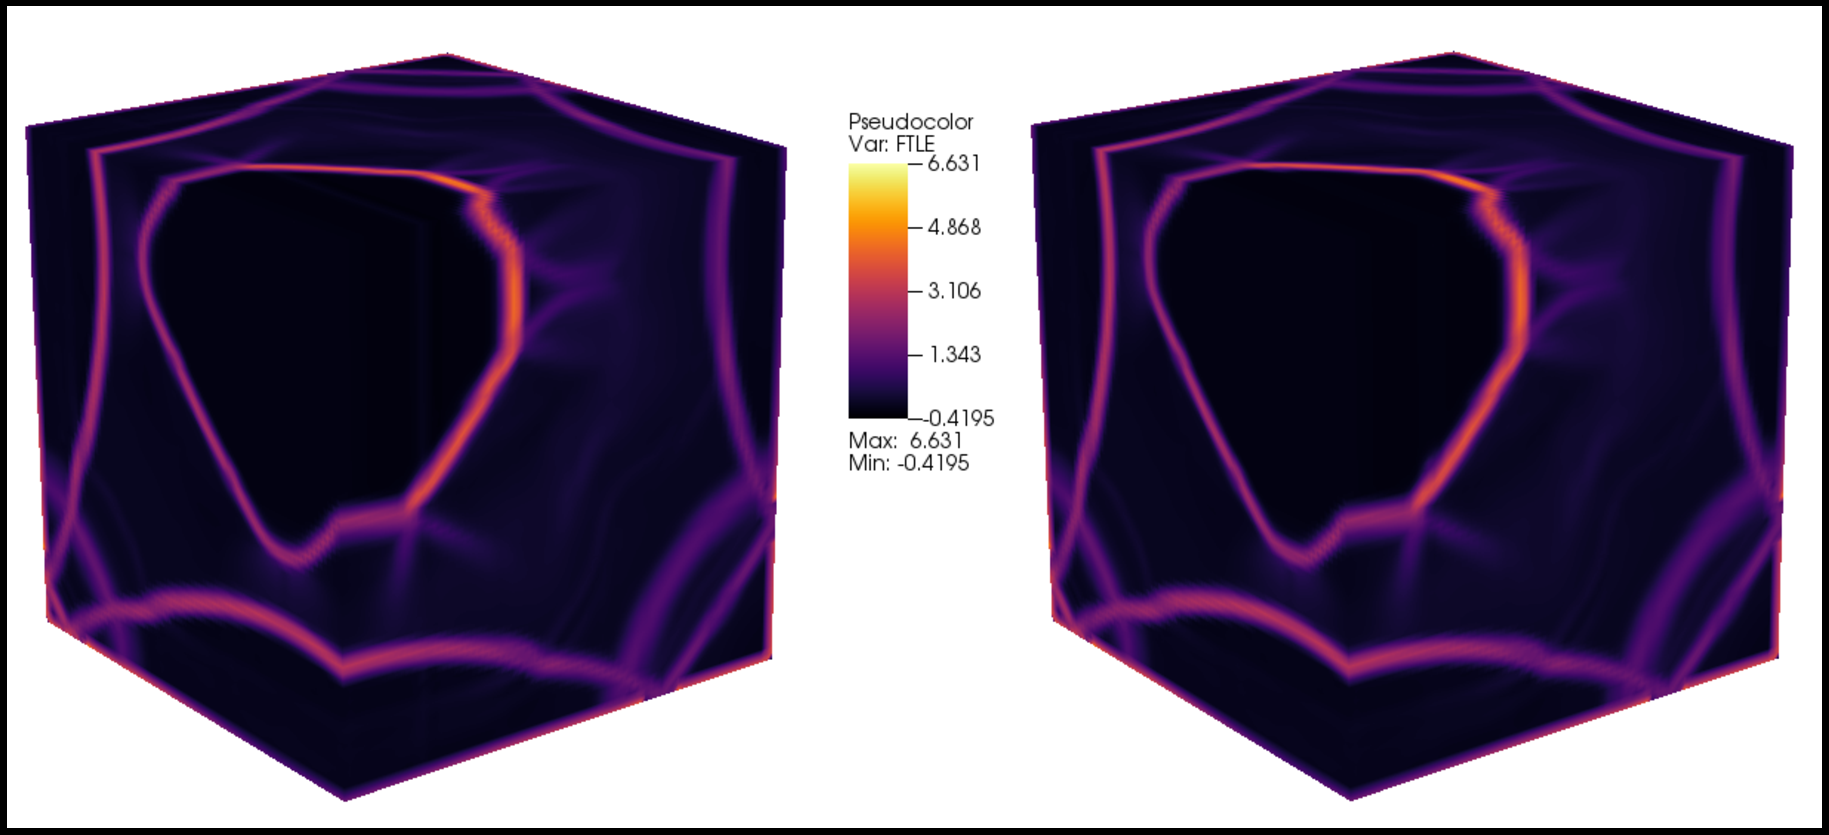
\includegraphics[width=0.85\linewidth,keepaspectratio]{Images/clover_ftle.pdf}
%\vspace{-3mm}
%\caption{Cloverleaf3D~(T8)}
%\label{clover_ftle}
%\end{subfigure}
\vspace{1mm}
\begin{subfigure}{\linewidth}
\centering
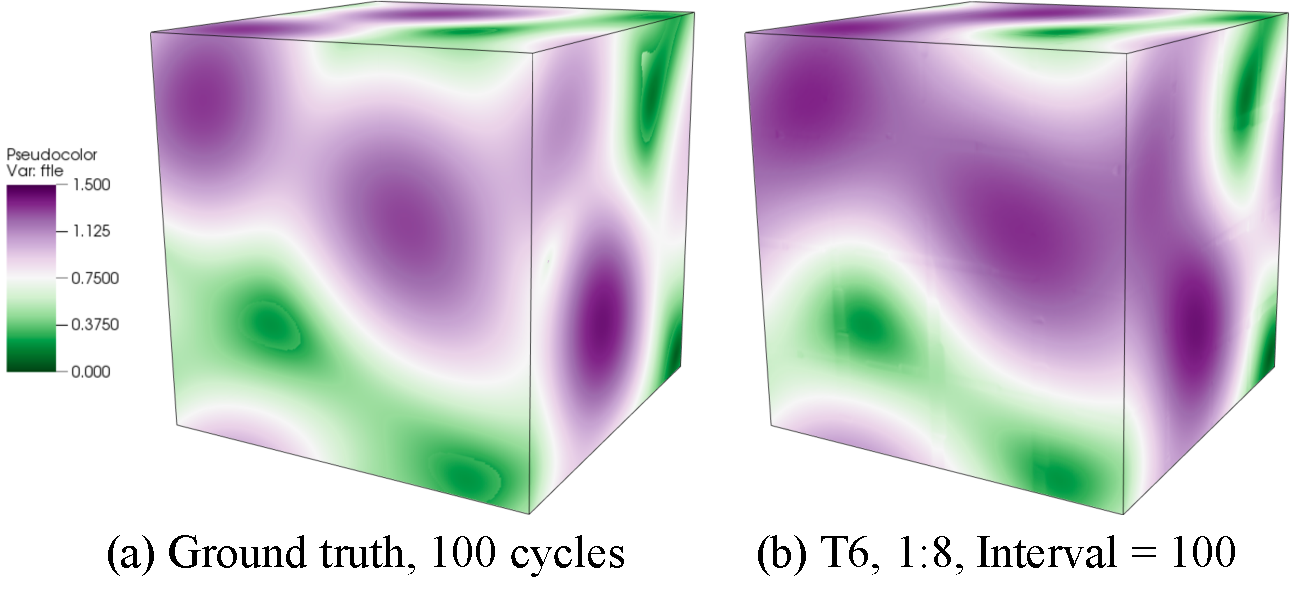
\includegraphics[width=0.85\linewidth,keepaspectratio]{Images/abc_ftle_new3.pdf}
\vspace{-3mm}
\caption{ABC~(T6)}
\label{abc_ftle}
\end{subfigure}
\vspace{1mm}
\begin{subfigure}{\linewidth}
\centering
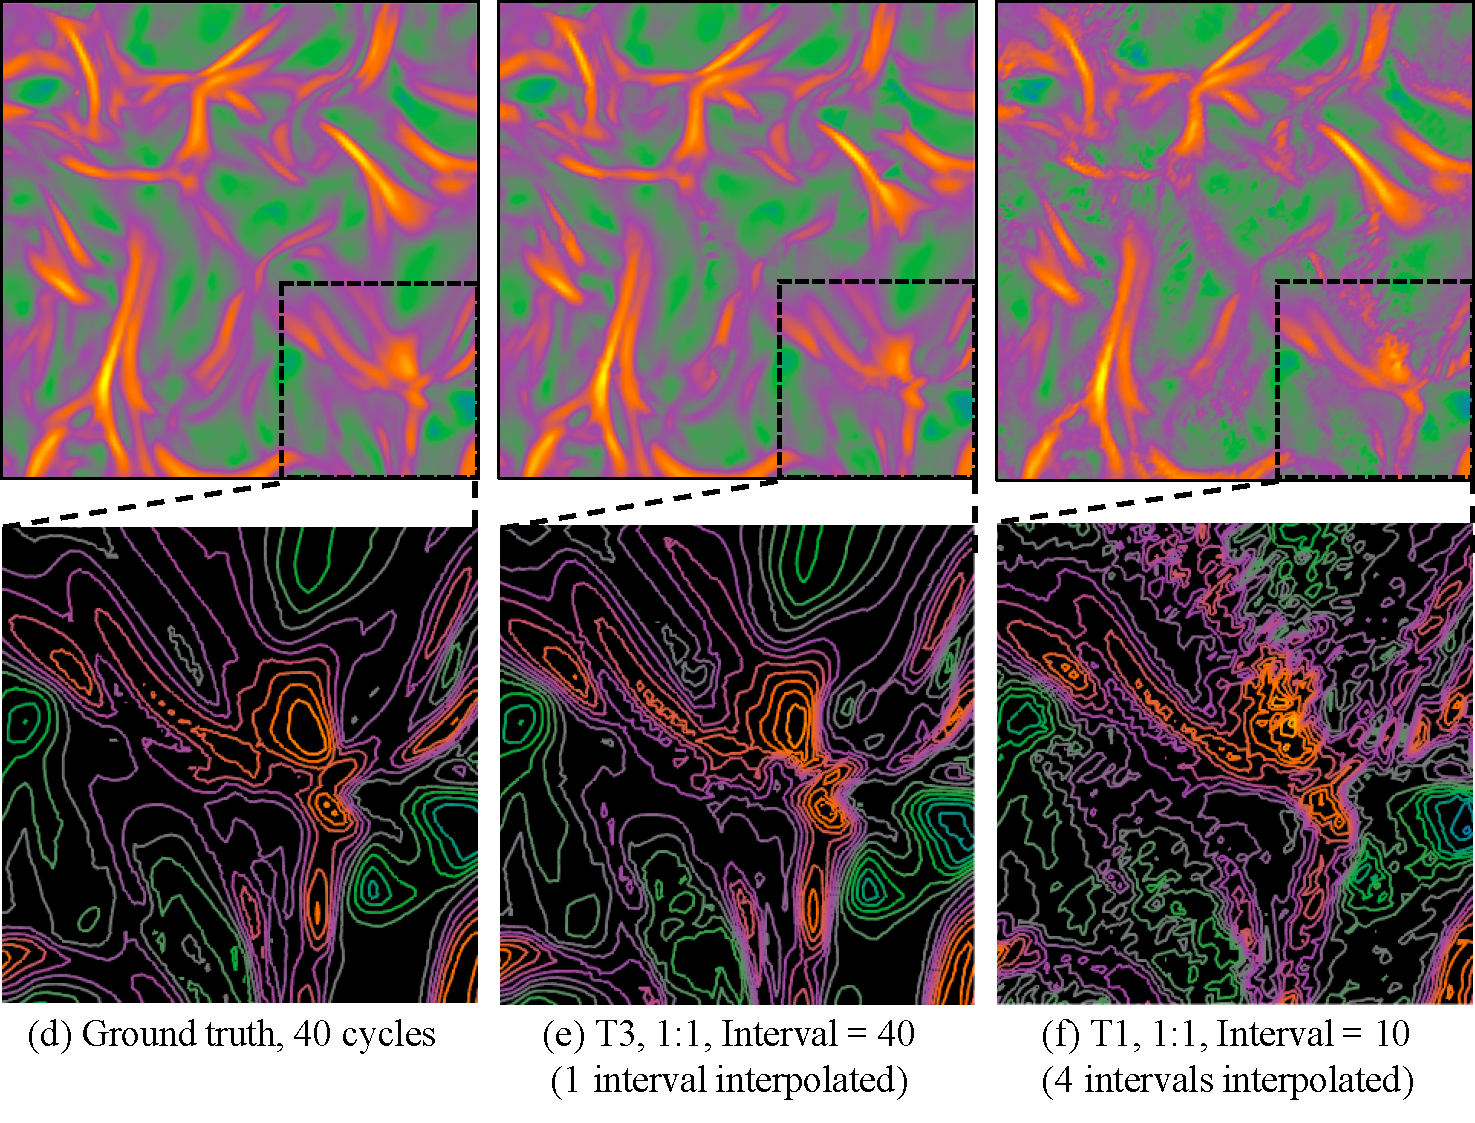
\includegraphics[width=0.9\linewidth,keepaspectratio]{Images/nyx_ftle_new2.pdf}
\vspace{-3mm}
\caption{Nyx~(T1)}
\label{nyx_ftle}
\end{subfigure}
\vspace{1mm}
\begin{subfigure}{\linewidth}
\centering
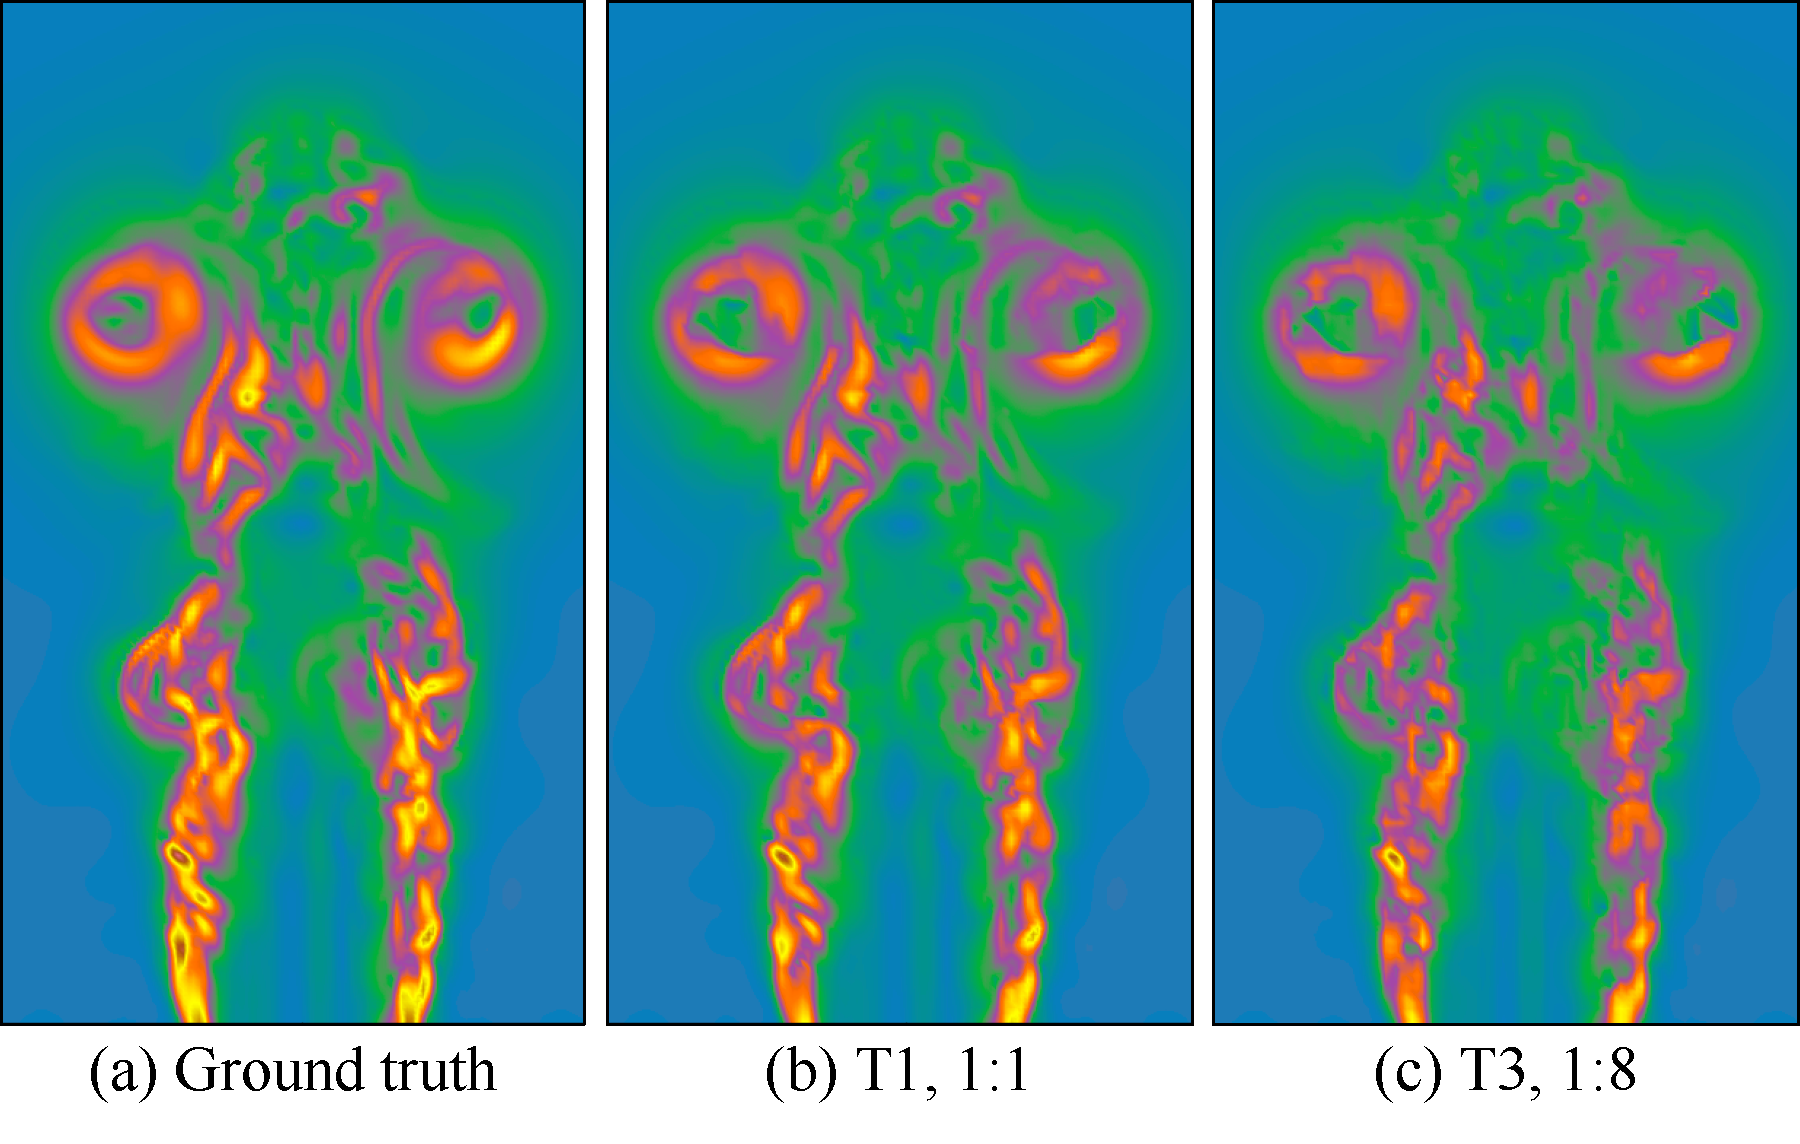
\includegraphics[width=0.9\linewidth,keepaspectratio, trim={0cm, 0cm, 0cm, 1cm}, clip]{Images/jet_ftle_new.pdf}
\vspace{-3mm}
\caption{Jet~(T2)}
\label{jet_ftle}
\end{subfigure}
\vspace{1mm}
\caption{\fix{A visual comparison of colormapped surfaces of subvolumes of FTLE scalar fields generated post hoc using the flow maps of Lagrangian$_{Dist}$~(left) and Lagrangian$_{Local}$~(right). Ridges in the FTLE field (identified by high scalar values), are used to visualize regions of interest. Cyan boxes highlight visible instances of difference in the output.}}
%\caption{A comparison of FTLE fields derived from the flow maps generated by Lagrangian$_{Dist}$~(left) and Lagrangian$_{Local}$~(right). Cyan boxes highlight instances of difference in the output.}
%\caption{Flow visualizations~(FTLE) generated using Lagrangian$_{Dist}$~(left) and Lagrangian$_{Local}$~(right) flow maps. Cyan boxes highlight instances of difference in the output.}
%\caption{Qualitative comparison of post hoc FTLE visualizations for the data sets considered.}
\label{fig:ftle_visualizations}
\vspace{-6mm}
\end{figure}
